\documentclass{beamer}\usepackage[]{graphicx}\usepackage[]{xcolor}
% maxwidth is the original width if it is less than linewidth
% otherwise use linewidth (to make sure the graphics do not exceed the margin)
\makeatletter
\def\maxwidth{ %
  \ifdim\Gin@nat@width>\linewidth
    \linewidth
  \else
    \Gin@nat@width
  \fi
}
\makeatother

\definecolor{fgcolor}{rgb}{0.345, 0.345, 0.345}
\newcommand{\hlnum}[1]{\textcolor[rgb]{0.686,0.059,0.569}{#1}}%
\newcommand{\hlstr}[1]{\textcolor[rgb]{0.192,0.494,0.8}{#1}}%
\newcommand{\hlcom}[1]{\textcolor[rgb]{0.678,0.584,0.686}{\textit{#1}}}%
\newcommand{\hlopt}[1]{\textcolor[rgb]{0,0,0}{#1}}%
\newcommand{\hlstd}[1]{\textcolor[rgb]{0.345,0.345,0.345}{#1}}%
\newcommand{\hlkwa}[1]{\textcolor[rgb]{0.161,0.373,0.58}{\textbf{#1}}}%
\newcommand{\hlkwb}[1]{\textcolor[rgb]{0.69,0.353,0.396}{#1}}%
\newcommand{\hlkwc}[1]{\textcolor[rgb]{0.333,0.667,0.333}{#1}}%
\newcommand{\hlkwd}[1]{\textcolor[rgb]{0.737,0.353,0.396}{\textbf{#1}}}%
\let\hlipl\hlkwb

\usepackage{framed}
\makeatletter
\newenvironment{kframe}{%
 \def\at@end@of@kframe{}%
 \ifinner\ifhmode%
  \def\at@end@of@kframe{\end{minipage}}%
  \begin{minipage}{\columnwidth}%
 \fi\fi%
 \def\FrameCommand##1{\hskip\@totalleftmargin \hskip-\fboxsep
 \colorbox{shadecolor}{##1}\hskip-\fboxsep
     % There is no \\@totalrightmargin, so:
     \hskip-\linewidth \hskip-\@totalleftmargin \hskip\columnwidth}%
 \MakeFramed {\advance\hsize-\width
   \@totalleftmargin\z@ \linewidth\hsize
   \@setminipage}}%
 {\par\unskip\endMakeFramed%
 \at@end@of@kframe}
\makeatother

\definecolor{shadecolor}{rgb}{.97, .97, .97}
\definecolor{messagecolor}{rgb}{0, 0, 0}
\definecolor{warningcolor}{rgb}{1, 0, 1}
\definecolor{errorcolor}{rgb}{1, 0, 0}
\newenvironment{knitrout}{}{} % an empty environment to be redefined in TeX

\usepackage{alltt}
\usepackage{graphicx}
\usepackage{amssymb}
\usepackage{pifont}
\usepackage{graphicx}
\usepackage{verbatim}
\usepackage{etoolbox}
\usepackage{everysel}
% \usepackage{enumitem}

%% This package allows text highlighting
\usepackage{soul}

%% This sets the theme of the presentation which controls
%% the formatting of the slides
\usetheme{Boadilla}

%% Turn off the navigation symbols
\setbeamertemplate{navigation symbols}{} 

%% Change the default itemize [ball]s to [circle]s
\setbeamertemplate{itemize items}[circle]

%% Change the default enumerate [ball]s to plain text
\setbeamertemplate{enumerate items}[default]

%% Load the enumitem package and ensure it works nicely with beamer
% \setitemize{label=\usebeamerfont*{itemize item}
%   \usebeamercolor[fg]{itemize item}
%   \usebeamertemplate{itemize item}}
% \setenumerate{label=\usebeamerfont*{enumerate item}
%   \usebeamercolor[fg]{enumerate item}
%   \usebeamertemplate{enumerate item}}

%% Set the author block so STATS 201/8 appears on every
\author{STATS 201/8}

%% Clear the date block
\date{}


\setbeamercolor{title}{bg=blue!40}
\setbeamerfont{title}{size=\LARGE,series=\bfseries}

%%Sectioning commands
\setbeamercolor{section title}{bg=blue!20}
\setbeamerfont{section title}{size=\large}

\setbeamertemplate{section page}{%
    \begingroup
        \begin{beamercolorbox}[sep=10pt,center,rounded=true,shadow=true]{section title}
        \usebeamerfont{section title}Section~\thechapter.\thesection \newline \insertsection\par
        \end{beamercolorbox}
		\vfill
    \endgroup
}

\newcommand{\BeginSection}[1]{\section{#1} \frame{\sectionpage}}
%\AtBeginSection[]{%
%    \begin{frame}
%        \sectionpage
%    \end{frame}
%}


%% This makes all equations blue
\AtBeginEnvironment{equation*}{\color{blue}}
\AtBeginEnvironment{align*}{\color{blue}}
\everymath{\color{blue}}

%% This puts a 0 point space between paragraphs, means we don't need to use vspace, or list environments if 
%% we don't want to
\setlength{\parskip}{0pt}


%% Russell: removes spaces after R input/output?
\setlength{\topsep}{0.5mm}

%% David: In addition to Russel's command to remove spaces after R input/output, these commands remove the space between R input/output.
%% Stackoverflow link: https://stackoverflow.com/questions/35734525/reduce-space-between-code-chunks-and-code-output-in-rmarkdown-beamer-presentatio
%% \setlength{\OuterFrameSep}{-2pt}
\makeatletter
\preto{\@verbatim}{\topsep=-1pt \partopsep=-1pt }
\makeatother

%% Some useful colors
\definecolor{darkgreen}{rgb}{0.176,0.486,0.031}
\definecolor{redbrown}{HTML}{950605}
\definecolor{darkred}{HTML}{d80605}


%% nice little macro for changing the font of R code
\newcommand{\rcode}[1]{\protect{\color{darkgreen}\texttt{#1}}}

%% macro for bold blue italics
\newcommand{\blueBoldEmph}[1]{{\color{blue}\textbf{\emph{#1}}}}

% ~iid macro
\newcommand{\iid }{\stackrel{iid}{\sim}}

%% Macro for t-test amd P-value
\newcommand{\ttest}{\emph{t}-test}
\newcommand{\pval}{\emph{P}-value}

%% Statistics operators 
\DeclareMathOperator{\Bias}{Bias}
\DeclareMathOperator{\Cov}{Cov}
\DeclareMathOperator*{\Cor}{Cor}
\DeclareMathOperator{\E}{E}
\DeclareMathOperator{\MSE}{MSE}
\DeclareMathOperator{\Odds}{Odds}
\DeclareMathOperator{\OR}{OR}
\DeclareMathOperator{\PMSE}{PMSE}
\DeclareMathOperator{\sd}{sd}
\DeclareMathOperator{\se}{se}
\DeclareMathOperator*{\Var}{Var}
\DeclareMathOperator{\logit}{logit}

%% Should see if can make this a mathop
\newcommand{\comb}[2]{\mbox{$\big(_{#2}^{#1}\big)$}}



\IfFileExists{upquote.sty}{\usepackage{upquote}}{}
\begin{document}
\newcommand{\thechapter}{15}


\newcommand{\cmark}{\ding{51}}
\newcommand{\xmark}{\ding{55}}

% \DeclareMathOperator{\E}{{E}}
% \DeclareMathOperator{\Var}{{Var}}

%% Sets the document title 
\title{Chapter \thechapter: \\ Modelling proportion data using the binomial distribution}
\institute{University of Auckland}

%\setlength{\topsep}{0mm} %Remove space before R output





\begin{frame}
\titlepage
\end{frame}


\begin{frame}[t]
\frametitle{Learning outcomes}
In this chapter you will learn about:
\begin{center}
\vspace{16pt}
\begin{minipage}{0.9\textwidth}
  \begin{itemize}
    \item Binary (Bernoulli) data, odds and log-odds
    \item Modelling log-odds
    \item Modelling the response when it is binary (ungrouped data) via \rcode{glm}
    \item Modelling the response when it is binomial (grouped binary data) via \rcode{glm}
    \item Example 1: Space shuttle {\em Challenger} accident
    \item Example 2: Probability of retaining fish in a trawl
    \item Relevant \rcode{R}-code.
  \end{itemize}
\end{minipage}
\end{center}
\end{frame}



%%%%%%%%%%%%%%%%%%%%%%%%%%%%%%%%%%%%%%%%%%%%%%%%%%%%%%%%%%%%%%%%%%%%%%%%%%%%%%%%%%%%%%%%%%%
\BeginSection{Binary (Bernoulli) data, odds and log-odds }
%%%%%%%%%%%%%%%%%%%%%%%%%%%%%%%%%%%%%%%%%%%%%%%%%%%%%%%%%%%%%%%%%%%%%%%%%%%%%%%%%%%%%%%%%%%



\begin{frame}
\frametitle{Binary (Bernoulli) data}
Here we are considering the situation where the response can only take \textbf{two} possible values. These might be coded in the form of:
\begin{itemize} \setlength{\itemsep}{2mm}
\item Zeros or ones. 
\item \rcode{TRUE} or \rcode{FALSE}. 
\item \rcode{Yes} or \rcode{No}.
\item \rcode{Success} or \rcode{Failure}..
\item Or any other pair of categorical values. 
\end{itemize}
\medskip

This is called a binary response and can be modelled using the \textbf{Bernoulli} distribution. 
\medskip

A Bernoulli distribution is just the special case of the binomial distribution\footnote{Recall, the binomial models the number of ``successes'' out of a fixed number of Bernoulli trials.} 
\end{frame}


\begin{frame}
\frametitle{Binary (Bernoulli) data\ldots}
\framesubtitle{Examples}
A Bernoulli random variable is the outcome for a single trial expressed as a 0 or 1, E.g.,
\medskip

\begin{itemize}
\item Whether or not I get a heads when I flip a coin.
\item Whether or not I roll a six with a six-sided dice.
\item Whether or not a soccer player scores a penalty kick.
\item Whether or not I score a shot in basketball.
\item Whether or not a green light is observed at a single set of traffic lights
on my regular commute to work.
\item Whether or not a patient survives an experimental procedure.
\end{itemize}
\medskip

In each of these examples we get to choose which outcomes are assigned the values 0 or 1.
\medskip

Typically, 0 = ``No'' (or ``Failure''), and 1 = ``Yes'' (or ``Success'').
\end{frame}


\begin{frame}
\frametitle{Bernoulli random variables}
If $Y$ is a Bernoulli random variable with parameter $p$, then $Y$ will take the value 1 with probability $p$, and the value 0 with probability $1-p$. %, i.e.
% \[
% \Pr(Y = y) = \begin{cases}
% p, &y = 1 \\
% 1 - p, & y=0\\
% \end{cases}
% \]

\medskip

Since it is a probability, $p$ must be a value that is between 0 and 1, i.e. $p \in [0, 1]$.

\medskip \medskip

For Bernoulli trials, the usual terminology is to refer to $Y$ as the
number of successes, either \textbf{zero} or \textbf{one}, from a single trial. 
\bigskip

It is easy to show\footnote{See STATS 210.} that the mean of a Bernoulli random variable is
\[
\E[Y]=p
\]
and that the variance is
\[
\Var(Y)=p (1-p)
\]

\end{frame}


\begin{frame}
% \frametitle{The Logit Function}
\frametitle{Odds}
We will soon be modelling Bernoulli data using the \rcode{glm} function. To be able to make sense of the fitted model we first need to know about {\bf odds}. 

The odds of an event occurring is given by
\[
\text{Odds} = \frac{\text{probability~event~occurs}}{\text{probability ~event~does~not~occur}}~=~\frac{\Pr(Y=1)}{\Pr(Y=0)}~ = ~\frac{p}{1-p}
\]

Note that $\text{Odds}$ must be a value between 0 to infinity, i.e. $\text{Odds} \in [0, \infty)$.
\medskip \medskip 

A little of bit of calculus gives us 
\[
p = \frac{\text{Odds}}{\text{Odds}+1}
\]

So, if we know the odds of an event then we also know the probability of that event (and vice-versa).
\end{frame}


\begin{frame}
\frametitle{What's the odds?}
The definition of odds is given in the previous slide.
\medskip

Luckily for us, the above definition of odds
has exactly the same meaning that we give to the word ``odds'' when we use it in
everyday speech when we use ``odds'' to describe how likely an event is to occur.
\bigskip

By way of example, let event A=\{I get an A- or better in STATS 201\}.
\medskip

\begin{itemize}
\item If the odds of A are 1 (i.e., 1-1, or even odds) then we are saying that
A is as likely to occur as not. That is Pr(A)=0.5, and Pr(not A)=0.5.
\item If the odds of A are 2 (i.e., 2-to-1) then we are saying that A is twice as likely to occur as not. That is Pr(A)=2/3 and Pr(not A)=1/3.
\item If the odds of A are 0.25 (i.e., 0.25-to-1) then we are saying that A is only 1/4
as likely to occur as not. That is Pr(A)=1/5 and Pr(not A)=4/5.
\end{itemize}
\end{frame}



\begin{frame}
\frametitle{Log-odds}

The logarithm of the odds (the log-odds for short) is
\[
\text{Log-Odds} = \log(\text{Odds}) = \log\left(\frac{p}{1-p}\right) \equiv \logit(p)
\]
Note that the log-odds (as a function of $p$) is called the \emph{logit} function.

Also, since $\text{Odds} \in [0,\infty)$ it follows that $\text{Log-Odds}$ can take any value on the real line, i.e. $\text{Log-Odds} \in (-\infty,+\infty)$.
\medskip

If we know the log-odds, then we can calculate $p$ using the following:
\[
p = \frac{\exp(\text{Log-Odds})}{1 + \exp(\text{Log-Odds})}
\]
This is called the \emph{logistic} function, and is well-known in mathematics as a function which maps the interval $(-\infty,+\infty)$ to $[0,1]$. In \rcode{R} it is the \rcode{plogis}\footnote{\rcode{plogis} is so named because it calculates the probability distribution function of the logistic distribution. This is precisely the logistic function.} function.
\end{frame}


%%%%%%%%%%%%%%%%%%%%%%%%%%%%%%%%%%%%%%%%%%%%%%%%%%%%%%%%%%%%%%%%%%%%%%%%%%%%%%%%%%%%%%%%%%%
\BeginSection{Modelling log-odds}
%%%%%%%%%%%%%%%%%%%%%%%%%%%%%%%%%%%%%%%%%%%%%%%%%%%%%%%%%%%%%%%%%%%%%%%%%%%%%%%%%%%%%%%%%%%

% Wouldn't it be cool if we could find some function $g()$ that allowed us to relate $\E[Y]$ to a linear function of some explanatory variables? I.e. so that
% \[
% g(E[Y]) = \beta_0 + \beta_1X_1+\beta_2X_2 + \cdots + \beta_pX_p \]


\begin{frame}
\frametitle{Why log-odds?}
Our aim in this Chapter is to be able to fit models for binary data that allow the probability of success, $p$, to depend on explanatory variables. This is equivalent to allowing the odds or log-odds to depend on the explanatory variables.
\medskip

For example, if $x$ is a numeric explanatory variable then we have the following modelling options:
\medskip

\begin{itemize}
  \item $p = \beta_0 + \beta_1  x$
  \item $\text{Odds} = \beta_0 + \beta_1 x$
  \item $\text{Log-Odds} = \beta_0 + \beta_1 x$
\end{itemize}
\medskip

Which would your suggest, and why?

\end{frame}


\begin{frame}
\frametitle{Why log-odds?\ldots}
Since our model places no restrictions\footnote{i.e., $\beta_0 \in (-\infty,\infty), \beta_1 \in (-\infty,\infty)$} on the values of $\beta_0$ or $\beta_1$, it is the case that $\beta_0 + \beta_1 x$ can take any value on the real line. 
\medskip

That is, $\beta_0 + \beta_1 x \in (-\infty,\infty)$.

\bigskip

\begin{itemize}
  \item $p = \beta_0 + \beta_1 x$ \xmark \\
  $p$ must be between 0 and 1. \medskip
    
  \item $\text{Odds} = \beta_0 + \beta_1 x$ \xmark \\
  $\text{Odds}$ must be between 0 and infinity. \medskip
    
  \item $\text{Log-Odds} = \beta_0 + \beta_1 x$ \cmark \\
  $\text{Log-Odds}$ can be any real number.
\end{itemize}

\end{frame}


\begin{frame}
\frametitle{Modelling log-odds}
We shall apply our linear model to the log-odds, and so our general form of the model is:
\[
\begin{split}
\log(\text{Odds}) &= \logit(p) \\
                  &= \logit(\mu) \\
                  &= \logit(E[Y|x_1 \ldots]) \\
                  &= \beta_0 + \beta_1 x_1  + \dots  
\end{split}
\]
\bigskip 

{\bf Remark:} This is analogous to what we did when the response variable was Poisson count data.
There we were using the model
\[ \log(\mu) = \log( E[Y|x_1 \ldots] ) = {\beta_0 + \beta_1 x_1 + \dots} \]
and note that $\log(\mu) \in (-\infty,\infty)$.
\end{frame}



\begin{frame}
\frametitle{Modelling log-odds\ldots}
\framesubtitle{With a single numeric explanatory variable}
When we have just a single explanatory variable $x$ that is numeric 
(i.e., not a factor) then the linear model for log-odds is:
\[ \log(\text{Odds}) = \beta_0 + \beta_1 x \]

In other words,
\[ \log \left( \frac{p}{1-p} \right) = \beta_0 + \beta_1 x  \]
where $p$ is the probability of ``success'' for a subject with explanatory variable $x$.

This can be re-arranged in the logistic form
\[ p= \frac{\exp(\beta_0 + \beta_1 x)}{1+exp(\beta_0 + \beta_1 x)} \]
This equation forms an ``S'' shaped curve as a function of $x$.
\end{frame}


\begin{frame}[fragile]
\frametitle{Modelling log-odds\ldots}
\framesubtitle{With a single continuous explanatory variable\ldots}
For example, 
if $\beta_0=-10$ and $\beta_1=0.3$ then the curve looks like:

% \vspace{-11mm}


\begin{figure}
  \centering
  \includegraphics{figure/RC-H15-002}
\end{figure}

\begin{itemize}
\item The greater the magnitude of $\beta_1$ the steeper the curve.\\
\item If $\beta_1<0$ the curve is a reverse ``S'' shape.\\
\item Changing $\beta_0$ changes the horizontal position of the curve.
\end{itemize}

\end{frame}


\begin{frame}
\frametitle{Logistic regression}
\begin{itemize}\setlength{\itemsep}{4mm}
\item The logistic function gives its name to this approach for modelling binary data -- it is commonly called \emph{logistic} regression. 
\item At the moment we are going to use logistic regression to model binary (\emph{Bernoulli}) data, 
but it can also be used to model proportion data in the form of the number of ``successes'' divided by the number of trials. The number of ``successes'' is assumed to be binomially distributed, so logistic regression is often called a binomial GLM. 
\item In GLMs, the function that links $\mu$ to the linear predictor is called the \emph{link} function. Here, $\mu=p$, and so the link function is the logit.
\end{itemize}

\end{frame}



%%%%%%%%%%%%%%%%%%%%%%%%%%%%%%%%%%%%%%%%%%%%%%%%%%%%%%%%%%%%%%%%%%%%%%%%%%%%%%%%%%%%%%%%%%%
\BeginSection{Modelling the response when it is binary \newline (ungrouped data) via \rcode{glm}}
%%%%%%%%%%%%%%%%%%%%%%%%%%%%%%%%%%%%%%%%%%%%%%%%%%%%%%%%%%%%%%%%%%%%%%%%%%%%%%%%%%%%%%%%%%%



\begin{frame}
\frametitle{Example -- Basketball}
A few years ago the lecturer of an experimental design course conducted a basketball shooting experiment in class. In this experiment
\begin{itemize}
  \item there were ten females and ten males;
  \item each shooter shot at the basket from 1m, 2m and 3m;
  \item each person took one shot from each distance;
  \item the order of the shooting distance was randomly chosen, and 
\item a \rcode{1} was recorded if the shot was successful, and a \rcode{0} was recorded if the shot was missed.
\end{itemize}

\medskip

What do \textbf{you} think is the most important factor affecting the probability of making the shot in this experiment?
\end{frame}



\begin{frame}[fragile]
\frametitle{Inspect the data}
\framesubtitle{Ungrouped format}
The data are read in to dataframe \rcode{bb.df}. It contains 60 observations, since each of the 20 students takes 3 shots.

\begin{knitrout}\scriptsize
\definecolor{shadecolor}{rgb}{0.969, 0.969, 0.969}\color{fgcolor}\begin{kframe}
\begin{alltt}
\hlstd{> }\hlstd{bb.df} \hlkwb{=} \hlkwd{read.csv}\hlstd{(}\hlstr{"Data/basketball.csv"}\hlstd{)}
\hlstd{> }\hlkwd{head}\hlstd{(bb.df,} \hlnum{10}\hlstd{)}
\end{alltt}
\begin{verbatim}
   distance gender basket
1         3      M      1
2         1      F      1
3         2      M      1
4         3      M      0
5         1      M      1
6         2      F      1
7         2      F      1
8         1      F      1
9         3      F      0
10        1      F      1
\end{verbatim}
\end{kframe}
\end{knitrout}
\bigskip

These data are in an \emph{ungrouped} format as the response variable for each row is either a success or a failure (a 1 or a 0).

\end{frame}


\begin{frame}[fragile]
\frametitle{Basketball}
\framesubtitle{Grouped format}
Because the ungrouped responses are zeros and ones, it is hard to detect patterns in this kind of data. However we can group the data over each combination of gender and distance. 
\medskip

The \rcode{xtabs} function produces a cross-tabulation table\footnote{Also called a frequency table.}

\begin{knitrout}\scriptsize
\definecolor{shadecolor}{rgb}{0.969, 0.969, 0.969}\color{fgcolor}\begin{kframe}
\begin{alltt}
\hlstd{> }\hlstd{success.tbl} \hlkwb{=} \hlkwd{xtabs}\hlstd{(basket}\hlopt{~}\hlstd{distance}\hlopt{+}\hlstd{gender,} \hlkwc{data} \hlstd{= bb.df)}
\hlstd{> }\hlstd{success.tbl}
\end{alltt}
\begin{verbatim}
        gender
distance  F  M
       1 10 10
       2  6  5
       3  2  1
\end{verbatim}
\end{kframe}
\end{knitrout}
Our conclusions should be kind of obvious from the table in this example, even without the model fitting.
\end{frame}


\begin{frame}[fragile]
\frametitle{Basketball\ldots}
\framesubtitle{Logistic regression model formula}
We want to fit a model that estimates how the probability of scoring is related to distance (numeric explanatory) and gender (factor explanatory). The interaction model (Chapter 8) is
\[
\begin{split}
\logit(p_i) &= \log\left(\frac{p_i}{1 - p_i}\right) \\
            &= \beta_0 + \beta_1 distance_i + \beta_2 gender_i + \beta_3 (gender_i \times distance_i)
\end{split}
\]

or in terms of $p_i$\footnote{We do not recommend that you try to write it this way in a test or assignment!}
\[
p_i = \frac{exp(\beta_0 + \beta_1 distance_i + \beta_2 gender_i + \beta_3 (gender_i \times distance_i))}{1 + exp(\beta_0 + \beta_1 distance_i + \beta_2 gender_i + \beta_3 (gender_i \times distance_i))}
\]

with $Y_i \sim \text{Bernoulli}(p_i)$ and $gender_i$ is an indicator variable which is 0 if the shooter is female, and 1 if the shooter is male.

\vspace{1em}

\end{frame}


\begin{frame}[fragile]
\frametitle{Basketball\ldots}
\framesubtitle{Fit the model\ldots}
Fitting the logistic regression model is easy.
\medskip

We simply tell the \rcode{glm} function that the responses are Bernoulli random variables by setting \rcode{family = binomial}.\footnote{Recall, the Bernoulli distribution is a special case of the binomial distribution.}

\medskip

\begin{knitrout}\scriptsize
\definecolor{shadecolor}{rgb}{0.969, 0.969, 0.969}\color{fgcolor}\begin{kframe}
\begin{alltt}
\hlstd{> }\hlstd{bb.fit} \hlkwb{=} \hlkwd{glm}\hlstd{(basket} \hlopt{~} \hlstd{distance} \hlopt{*} \hlstd{gender,} \hlkwc{family} \hlstd{= binomial,}
\hlstd{+ }             \hlkwc{data} \hlstd{= bb.df)}
\end{alltt}
\end{kframe}
\end{knitrout}

\medskip

Note that, as with Poisson GLMs, we \textbf{do not} transform the responses. 
\bigskip

{\bf Aside:} By default the \rcode{glm()} function uses the logit link function (i.e., does logistic regression) when we set \rcode{family = binomial}. Other choices are possible -- see STATS 730.
\end{frame}


\begin{frame}[fragile]
\frametitle{Basketball\ldots}
\framesubtitle{Check the model\ldots}
Model checking is difficult when the data are \emph{ungrouped}.\footnote{This is because the data are {\em sparse}, in the sense that they are either 0's or 1's.}

\begin{knitrout}\scriptsize
\definecolor{shadecolor}{rgb}{0.969, 0.969, 0.969}\color{fgcolor}\begin{kframe}
\begin{alltt}
\hlstd{> }\hlkwd{plot}\hlstd{(bb.fit,} \hlkwc{which} \hlstd{=} \hlnum{1}\hlstd{,} \hlkwc{lty}\hlstd{=}\hlnum{2}\hlstd{)}
\end{alltt}
\end{kframe}
\end{knitrout}

\begin{figure}
  \centering
  \includegraphics[scale=0.8]{figure/RC-H15-006}
\end{figure}

The plot of the residuals versus the fitted values is not particularly informative. Even if the model is appropriate, it can looked quite patterned. Influence checks are also of little use.
\end{frame}


\begin{frame}[fragile]
\frametitle{Basketball\ldots}
\framesubtitle{Inspect the fitted model}
\begin{knitrout}\scriptsize
\definecolor{shadecolor}{rgb}{0.969, 0.969, 0.969}\color{fgcolor}\begin{kframe}
\begin{alltt}
\hlstd{> }\hlkwd{summary}\hlstd{(bb.fit)}
\end{alltt}
\end{kframe}
\end{knitrout}

\begin{knitrout}\scriptsize
\definecolor{shadecolor}{rgb}{0.969, 0.969, 0.969}\color{fgcolor}\begin{kframe}
\begin{verbatim}
Call:
glm(formula = basket ~ distance * gender, family = binomial, 

Coefficients:
                 Estimate Std. Error z value Pr(>|z|)   
(Intercept)        5.5878     1.9050   2.933  0.00335 **
distance          -2.4159     0.8181  -2.953  0.00314 **
genderM            0.6710     2.9235   0.230  0.81847   
distance:genderM  -0.5668     1.3213  -0.429  0.66794   
---
(Dispersion parameter for binomial family taken to be 1)

    Null deviance: 82.108  on 59  degrees of freedom
Residual deviance: 46.202  on 56  degrees of freedom
\end{verbatim}
\end{kframe}
\end{knitrout}

When the data are \emph{ungrouped} we also {\bf cannot} use the residual deviance in the same way we did for Poisson GLMs.
\medskip

We just have to presume that the fitted model satisfies assumptions.
\end{frame}



\begin{frame}[fragile]
\frametitle{Basketball\ldots}
\framesubtitle{Simplify the model}
There is no evidence of an interaction between gender and distance. We'll apply Occam's razor and drop it from the model.
\bigskip

\begin{knitrout}\scriptsize
\definecolor{shadecolor}{rgb}{0.969, 0.969, 0.969}\color{fgcolor}\begin{kframe}
\begin{alltt}
\hlstd{> }\hlstd{bb.fit1} \hlkwb{=} \hlkwd{glm}\hlstd{(basket} \hlopt{~} \hlstd{distance} \hlopt{+} \hlstd{gender,} \hlkwc{family} \hlstd{= binomial,} \hlkwc{data} \hlstd{= bb.df)}
\hlstd{> }\hlkwd{summary}\hlstd{(bb.fit1)}
\end{alltt}
\end{kframe}
\end{knitrout}

\begin{knitrout}\scriptsize
\definecolor{shadecolor}{rgb}{0.969, 0.969, 0.969}\color{fgcolor}\begin{kframe}
\begin{verbatim}
Call:
glm(formula = basket ~ distance + gender, family = binomial, 

Coefficients:
            Estimate Std. Error z value Pr(>|z|)    
(Intercept)   6.1469     1.5242   4.033 5.51e-05 ***
distance     -2.6648     0.6364  -4.188 2.82e-05 ***
genderM      -0.5478     0.7486  -0.732    0.464    
---
(Dispersion parameter for binomial family taken to be 1)

    Null deviance: 82.108  on 59  degrees of freedom
Residual deviance: 46.392  on 57  degrees of freedom
\end{verbatim}
\end{kframe}
\end{knitrout}

Looks like we can drop gender, too.

\end{frame}


\begin{frame}[fragile]
\frametitle{Basketball\ldots}
\framesubtitle{Simplify the model\ldots}
\begin{knitrout}\scriptsize
\definecolor{shadecolor}{rgb}{0.969, 0.969, 0.969}\color{fgcolor}\begin{kframe}
\begin{alltt}
\hlstd{> }\hlstd{bb.fit2} \hlkwb{=} \hlkwd{glm}\hlstd{(basket} \hlopt{~} \hlstd{distance,} \hlkwc{family} \hlstd{= binomial,} \hlkwc{data} \hlstd{= bb.df)}
\hlstd{> }\hlkwd{summary}\hlstd{(bb.fit2)}
\end{alltt}
\end{kframe}
\end{knitrout}

\begin{knitrout}\scriptsize
\definecolor{shadecolor}{rgb}{0.969, 0.969, 0.969}\color{fgcolor}\begin{kframe}
\begin{verbatim}
Call:
glm(formula = basket ~ distance, family = binomial, data = bb.df)

Coefficients:
            Estimate Std. Error z value Pr(>|z|)    
(Intercept)   5.7980     1.4038   4.130 3.63e-05 ***
distance     -2.6310     0.6274  -4.193 2.75e-05 ***
---
(Dispersion parameter for binomial family taken to be 1)

    Null deviance: 82.108  on 59  degrees of freedom
Residual deviance: 46.937  on 58  degrees of freedom
\end{verbatim}
\end{kframe}
\end{knitrout}
\end{frame}



\begin{frame}[fragile]
\frametitle{Basketball\ldots}
\framesubtitle{Interpretting the fitted model}
\label{pg:Odds}
So, our final model is of the form
\[ \text{Log-Odds} = \beta_0 + \beta_1 \times distance \] 
This means that a 1 metre increase in distance increases the log-odds by $\beta_1$.
\bigskip

In terms of odds, we have
\[ 
\begin{split}
\text{Odds} &= \exp( \beta_0 + \beta_1 \times distance) \\
            &= \exp(\beta_0) \times \exp(\beta_1)^{distance} 
\end{split}
\] 
This means that a 1 metre increase in distance multiplies the odds by $\exp(\beta_1) $.           
\end{frame}



\begin{frame}[fragile]
\frametitle{Basketball\ldots}
\framesubtitle{Interpretting the fitted model\dots}




\begin{knitrout}\scriptsize
\definecolor{shadecolor}{rgb}{0.969, 0.969, 0.969}\color{fgcolor}\begin{kframe}
\begin{alltt}
\hlstd{> }\hlkwd{coef}\hlstd{(bb.fit2)}
\end{alltt}
\begin{verbatim}
(Intercept)    distance 
   5.797968   -2.631033 
\end{verbatim}
\end{kframe}
\end{knitrout}

The estimated coefficient on distance, $\hat\beta_1$, is -2.63. This says that the \emph{log-odds of success} decreases by 2.63 for every 1 metre increase of the shooter from the goal. 

\medskip

\begin{knitrout}\scriptsize
\definecolor{shadecolor}{rgb}{0.969, 0.969, 0.969}\color{fgcolor}\begin{kframe}
\begin{alltt}
\hlstd{> }\hlkwd{exp}\hlstd{(}\hlkwd{coef}\hlstd{(bb.fit2))}
\end{alltt}
\begin{verbatim}
 (Intercept)     distance 
329.62899018   0.07200401 
\end{verbatim}
\begin{alltt}
\hlstd{> }\hlnum{100}\hlopt{*}\hlstd{(}\hlnum{1}\hlopt{-}\hlkwd{exp}\hlstd{(}\hlkwd{coef}\hlstd{(bb.fit2)))}
\end{alltt}
\begin{verbatim}
(Intercept)    distance 
-32862.8990     92.7996 
\end{verbatim}
\end{kframe}
\end{knitrout}


\medskip

By exponentiating $\hat\beta_1$ we can now say that a 1 metre increase in the distance results multiplies the odds of shooting a basket by 0.072. However, it would be more natural to say that it results in a $100\times(1-0.072)\% = 92.8\%$ reduction in the odds. 

\end{frame}


\begin{frame}[fragile]
\frametitle{Basketball\ldots}
\framesubtitle{Interpretting the fitted model\ldots}
For our Executive Summaries we need confidence intervals rather than point estimates:
\medskip

\begin{knitrout}\scriptsize
\definecolor{shadecolor}{rgb}{0.969, 0.969, 0.969}\color{fgcolor}\begin{kframe}
\begin{alltt}
\hlstd{> }\hlstd{(bb.ci2} \hlkwb{=} \hlkwd{confint}\hlstd{(bb.fit2))}
\end{alltt}


{\ttfamily\noindent\itshape\color{messagecolor}{Waiting for profiling to be done...}}\begin{verbatim}
                2.5 %    97.5 %
(Intercept)  3.422396  9.037020
distance    -4.103523 -1.568945
\end{verbatim}
\begin{alltt}
\hlstd{> }\hlnum{100}\hlopt{*}\hlstd{(}\hlnum{1}\hlopt{-}\hlkwd{exp}\hlstd{(bb.ci2))}
\end{alltt}
\begin{verbatim}
                  2.5 %        97.5 %
(Intercept) -2964.27509 -840767.86136
distance       98.34856      79.17351
\end{verbatim}
\end{kframe}
\end{knitrout}

A 1 metre increase in the distance results in a reduction in the odds of scoring of between 79.2\% and 98.3\%

\end{frame}


\begin{frame}[fragile]
\frametitle{Estimating $p$}
\framesubtitle{Basketball example}
How do we estimate the probability of a successful shot from distances of 1, 2 and 3 m?
\medskip

By default, \rcode{predict} will give estimates on the log-odds scale, that is, it will calculate the linear predictor $\hat{\beta}_0+\hat{\beta}_1 \times distance$.

\begin{knitrout}\scriptsize
\definecolor{shadecolor}{rgb}{0.969, 0.969, 0.969}\color{fgcolor}\begin{kframe}
\begin{alltt}
\hlstd{> }\hlstd{predn.df}\hlkwb{=}\hlkwd{data.frame}\hlstd{(}\hlkwc{distance} \hlstd{=} \hlnum{1}\hlopt{:}\hlnum{3}\hlstd{)}
\hlstd{> }\hlstd{bb.logit.pred} \hlkwb{=} \hlkwd{predict}\hlstd{(bb.fit2,} \hlkwc{newdata} \hlstd{= predn.df)}
\hlstd{> }\hlstd{bb.logit.pred}
\end{alltt}
\begin{verbatim}
         1          2          3 
 3.1669343  0.5359009 -2.0951325 
\end{verbatim}
\end{kframe}
\end{knitrout}
We can easily convert this to the response (i.e., probability) scale

\begin{knitrout}\scriptsize
\definecolor{shadecolor}{rgb}{0.969, 0.969, 0.969}\color{fgcolor}\begin{kframe}
\begin{alltt}
\hlstd{> }\hlkwd{plogis}\hlstd{(bb.logit.pred)}
\end{alltt}
\begin{verbatim}
        1         2         3 
0.9595708 0.6308584 0.1095708 
\end{verbatim}
\end{kframe}
\end{knitrout}

Even easier is to use the \rcode{type="response"} argument of \rcode{predict}:
\begin{knitrout}\scriptsize
\definecolor{shadecolor}{rgb}{0.969, 0.969, 0.969}\color{fgcolor}\begin{kframe}
\begin{alltt}
\hlstd{> }\hlkwd{predict}\hlstd{(bb.fit2,} \hlkwc{newdata} \hlstd{= predn.df,} \hlkwc{type}\hlstd{=}\hlstr{"response"}\hlstd{)}
\end{alltt}
\begin{verbatim}
        1         2         3 
0.9595708 0.6308584 0.1095708 
\end{verbatim}
\end{kframe}
\end{knitrout}

\end{frame}



\begin{frame}[fragile]
\frametitle{Confidence Intervals for $p$}
\framesubtitle{Basketball example\ldots}
Confidence intervals need to first be calculated on the log-odds scale, and then transformed back to the probability scale.
\begin{knitrout}\scriptsize
\definecolor{shadecolor}{rgb}{0.969, 0.969, 0.969}\color{fgcolor}\begin{kframe}
\begin{alltt}
\hlstd{> }\hlstd{bb.logit.predses} \hlkwb{=} \hlkwd{predict}\hlstd{(bb.fit2,} \hlkwc{newdata} \hlstd{= predn.df,} \hlkwc{se.fit} \hlstd{=} \hlnum{TRUE}\hlstd{)}\hlopt{$}\hlstd{se.fit}
\hlstd{> }\hlstd{bb.logit.predses}
\end{alltt}
\begin{verbatim}
        1         2         3 
0.8151018 0.3812977 0.6432312 
\end{verbatim}
\begin{alltt}
\hlstd{> }\hlcom{# Lower and upper bounds of CIs for the log-odds}
\hlstd{> }\hlstd{lower} \hlkwb{=} \hlstd{bb.logit.pred} \hlopt{-} \hlnum{1.96}\hlopt{*}\hlstd{bb.logit.predses}
\hlstd{> }\hlstd{upper} \hlkwb{=} \hlstd{bb.logit.pred} \hlopt{+} \hlnum{1.96}\hlopt{*}\hlstd{bb.logit.predses}
\hlstd{> }\hlstd{ci} \hlkwb{=} \hlkwd{cbind}\hlstd{(lower, upper)}
\end{alltt}
\end{kframe}
\end{knitrout}
and convert these to probabilities:

\begin{knitrout}\scriptsize
\definecolor{shadecolor}{rgb}{0.969, 0.969, 0.969}\color{fgcolor}\begin{kframe}
\begin{alltt}
\hlstd{> }\hlkwd{plogis}\hlstd{(ci)}
\end{alltt}
\begin{verbatim}
       lower     upper
1 0.82768876 0.9915452
2 0.44733541 0.7830016
3 0.03370361 0.3027157
\end{verbatim}
\end{kframe}
\end{knitrout}

We see that the probability of a goal from 1 metre distance is between 0.828 and 0.991, but drops to between 0.034 and 0.303 at 3 metres.
\end{frame}


\begin{frame}[fragile]
\frametitle{Confidence Intervals for $p$ the easy way}
\framesubtitle{Basketball example\ldots}
Or we can use the \rcode{predictGLM} function from the \rcode{s20x} package.
\medskip

To get confidence intervals for log-odds
\begin{knitrout}\scriptsize
\definecolor{shadecolor}{rgb}{0.969, 0.969, 0.969}\color{fgcolor}\begin{kframe}
\begin{alltt}
\hlstd{> }\hlkwd{predictGLM}\hlstd{(bb.fit2,}\hlkwc{newdata} \hlstd{=} \hlkwd{data.frame}\hlstd{(}\hlkwc{distance} \hlstd{=} \hlnum{1}\hlopt{:}\hlnum{3}\hlstd{),}\hlkwc{type}\hlstd{=}\hlstr{"link"}\hlstd{)}
\end{alltt}


{\ttfamily\noindent\itshape\color{messagecolor}{***Estimates and CIs are on the link scale***}}\begin{verbatim}
         fit        lwr        upr
1  3.1669343  1.5693642  4.7645045
2  0.5359009 -0.2114289  1.2832308
3 -2.0951325 -3.3558424 -0.8344225
\end{verbatim}
\end{kframe}
\end{knitrout}
or to get confidence intervals for the probabilities
\begin{knitrout}\scriptsize
\definecolor{shadecolor}{rgb}{0.969, 0.969, 0.969}\color{fgcolor}\begin{kframe}
\begin{alltt}
\hlstd{> }\hlkwd{predictGLM}\hlstd{(bb.fit2,}\hlkwc{newdata} \hlstd{=} \hlkwd{data.frame}\hlstd{(}\hlkwc{distance} \hlstd{=} \hlnum{1}\hlopt{:}\hlnum{3}\hlstd{),}\hlkwc{type}\hlstd{=}\hlstr{"response"}\hlstd{)}
\end{alltt}


{\ttfamily\noindent\itshape\color{messagecolor}{***Estimates and CIs are on the response scale***}}\begin{verbatim}
        fit        lwr       upr
1 0.9595708 0.82769294 0.9915450
2 0.6308584 0.44733881 0.7829992
3 0.1095708 0.03370437 0.3027108
\end{verbatim}
\end{kframe}
\end{knitrout}
\bigskip

In the next section, we reproduce the above analysis after first grouping the data. 
\end{frame}



%%%%%%%%%%%%%%%%%%%%%%%%%%%%%%%%%%%%%%%%%%%%%%%%%%%%%%%%%%%%%%%%%%%%%%%%%%%%%%%%%%%%%%%%%%%
\BeginSection{Modelling the response when it is binomial \newline (grouped binary data) via \rcode{glm}}
%%%%%%%%%%%%%%%%%%%%%%%%%%%%%%%%%%%%%%%%%%%%%%%%%%%%%%%%%%%%%%%%%%%%%%%%%%%%%%%%%%%%%%%%%%%



\begin{frame}
\frametitle{The binomial distribution}

A binomial random variable is the number of successes that occur over a fixed number ($n$) of Bernoulli trials, all with the same probability of success ($p$):
\begin{itemize}
\item The number of heads if I flip a coin fifty times.
\item The number of sixes I get if I roll four dice.
\item The number of penalties a football team scores in a penalty shoot-out.
\item The number of successful basketball shots out of ten attempts.
\item The number of green lights out of the total number of traffic lights
on my regular commute to work.
\item The number of patients who survive an experimental procedure, 
out of the number that underwent that procedure.
\item The number of O-rings that fail when a space shuttle is launched, 
out of the total of six O-rings on the solid fuel rockets.
\end{itemize}

\bigskip

One difference between a binomial and Poisson random variable is that the binomial has an upper limit set by the number of trials.

\end{frame}


\begin{frame}[fragile]
\frametitle{Example revisited -- Basketball: Grouped data}
In many situations it is possible to format the binary data so that they are \emph{grouped}. 
\medskip

With grouped data, all trials with the same values of the explanatory variables are aggregated in the same row, along with the number of ``successes'' and ``failures''.
\medskip

We demonstrate with our basketball data:
\begin{knitrout}\scriptsize
\definecolor{shadecolor}{rgb}{0.969, 0.969, 0.969}\color{fgcolor}\begin{kframe}
\begin{alltt}
\hlstd{> }\hlcom{#Load dplyr package to manipulate data frames}
\hlstd{> }\hlkwd{library}\hlstd{(dplyr)}
\hlstd{> }\hlstd{bb.grouped.df} \hlkwb{=} \hlstd{bb.df} \hlopt \hlkwd{group_by}\hlstd{(gender,distance)} \hlopt
\hlstd{+ }                      \hlkwd{summarize}\hlstd{(}\hlkwc{n}\hlstd{=}\hlkwd{n}\hlstd{(),}\hlkwc{propn}\hlstd{=}\hlkwd{sum}\hlstd{(basket)}\hlopt{/}\hlstd{n)}
\hlstd{> }\hlcom{#Change tibble back to a data frame}
\hlstd{> }\hlstd{bb.grouped.df} \hlkwb{=} \hlkwd{data.frame}\hlstd{(bb.grouped.df)}
\hlstd{> }\hlstd{bb.grouped.df}
\end{alltt}
\begin{verbatim}
  gender distance  n propn
1      F        1 10   1.0
2      F        2 10   0.6
3      F        3 10   0.2
4      M        1 10   1.0
5      M        2 10   0.5
6      M        3 10   0.1
\end{verbatim}
\end{kframe}
\end{knitrout}
\end{frame}



\begin{frame}[fragile]
\frametitle{Basketball: Grouped data}
We can still use \rcode{glm} to fit a logistic regression model to grouped data.
\bigskip

Previously, we considered each of the 60 attempts to score as a separate Bernoulli trial.

\medskip

Instead, we now consider the number of successes out of 10 attempts at each level of gender and distance. This is a binomial random variable.
\bigskip

Both approaches will give you the same estimates, confidence intervals, and conclusions, but there are some advantages to having grouped data. Especially, being better able to check model assumptions.
\end{frame}



\begin{frame}[fragile]
\frametitle{Basketball: Grouped data\ldots}
\framesubtitle{Fitting the model}
We set the proportion of successes as the response, and use the argument \rcode{weights} to specify the number of trials associated with each observation.

\begin{knitrout}\scriptsize
\definecolor{shadecolor}{rgb}{0.969, 0.969, 0.969}\color{fgcolor}\begin{kframe}
\begin{alltt}
\hlstd{> }\hlstd{bb.fit3} \hlkwb{=} \hlkwd{glm}\hlstd{(propn} \hlopt{~} \hlstd{distance} \hlopt{*} \hlstd{gender,} \hlkwc{weights} \hlstd{= n,}
\hlstd{+ }              \hlkwc{family} \hlstd{= binomial,} \hlkwc{data} \hlstd{= bb.grouped.df)}
\hlstd{> }\hlkwd{summary}\hlstd{(bb.fit3)}
\end{alltt}
\end{kframe}
\end{knitrout}

\begin{knitrout}\scriptsize
\definecolor{shadecolor}{rgb}{0.969, 0.969, 0.969}\color{fgcolor}\begin{kframe}
\begin{verbatim}
Call:
glm(formula = propn ~ distance * gender, family = binomial, data = bb.grouped.df, 

Coefficients:
                 Estimate Std. Error z value Pr(>|z|)   
(Intercept)        5.5878     1.9050   2.933  0.00335 **
distance          -2.4159     0.8181  -2.953  0.00314 **
genderM            0.6710     2.9236   0.230  0.81848   
distance:genderM  -0.5668     1.3214  -0.429  0.66795   
---
(Dispersion parameter for binomial family taken to be 1)

    Null deviance: 38.2749  on 5  degrees of freedom
Residual deviance:  2.3688  on 2  degrees of freedom
\end{verbatim}
\end{kframe}
\end{knitrout}


\end{frame}



\begin{frame}[fragile]
\frametitle{Basketball: Grouped data\ldots}
\framesubtitle{Checking the model\ldots}

The grouped data output is equivalent to that from working with the \emph{ungrouped} data, except that the deviance values have changed.
\bigskip


We may now interpret residual plots and check the residual deviance statistic, notwithstanding that we ideally require the expected count of both successes and failures to be reasonably large, say $>5$.\footnote{This is not satisfied for the basketball data, but we will proceed anyway.}
\medskip

\begin{knitrout}\scriptsize
\definecolor{shadecolor}{rgb}{0.969, 0.969, 0.969}\color{fgcolor}\begin{kframe}
\begin{alltt}
\hlstd{> }\hlnum{1} \hlopt{-} \hlkwd{pchisq}\hlstd{(}\hlnum{2.3688}\hlstd{,} \hlnum{2}\hlstd{)}
\end{alltt}
\begin{verbatim}
[1] 0.3059297
\end{verbatim}
\end{kframe}
\end{knitrout}
\medskip

No problems with the residual deviance.
\end{frame}



\begin{frame}[fragile]
\frametitle{Basketball: Grouped data\ldots}
\framesubtitle{Checking the model\ldots}

\begin{knitrout}\scriptsize
\definecolor{shadecolor}{rgb}{0.969, 0.969, 0.969}\color{fgcolor}\begin{kframe}
\begin{alltt}
\hlstd{> }\hlkwd{plot}\hlstd{(bb.fit3,} \hlkwc{which} \hlstd{=} \hlnum{1}\hlstd{,} \hlkwc{lty}\hlstd{=}\hlnum{2}\hlstd{)}
\end{alltt}
\end{kframe}
\end{knitrout}
  
\begin{figure}
  \centering
  \includegraphics{figure/RC-H15-029}
\end{figure}

We only have six observations (one for each combination of distance and gender), so it is difficult to see if there is a pattern in the residuals, but in this case none are large enough to worry us.

The fitted model is not perfect, but should still be useful.
\end{frame}



\begin{frame}[fragile]
\frametitle{An alternative way to specify the model}
\framesubtitle{Basketball: Grouped data\ldots}
Sometimes the grouped data are provided as the number of successes and failures:
\bigskip

\begin{knitrout}\scriptsize
\definecolor{shadecolor}{rgb}{0.969, 0.969, 0.969}\color{fgcolor}\begin{kframe}
\begin{alltt}
\hlstd{> }\hlstd{bb.grouped.df} \hlkwb{=} \hlkwd{transform}\hlstd{(bb.grouped.df,} \hlkwc{success}\hlstd{=n}\hlopt{*}\hlstd{propn,} \hlkwc{fail}\hlstd{=n}\hlopt{*}\hlstd{(}\hlnum{1}\hlopt{-}\hlstd{propn))}
\hlstd{> }\hlstd{bb.grouped.df}
\end{alltt}
\begin{verbatim}
  gender distance  n propn success fail
1      F        1 10   1.0      10    0
2      F        2 10   0.6       6    4
3      F        3 10   0.2       2    8
4      M        1 10   1.0      10    0
5      M        2 10   0.5       5    5
6      M        3 10   0.1       1    9
\end{verbatim}
\end{kframe}
\end{knitrout}
\end{frame}


\begin{frame}[fragile]
\frametitle{An alternative way to specify the model\ldots}
\framesubtitle{Basketball: Grouped data\ldots}
Then, on the left-hand side of the model formula we provide \rcode{glm} with the names of the two columns containing the number of successes and failures, and omit the \rcode{weights} argument.
\bigskip

\begin{knitrout}\scriptsize
\definecolor{shadecolor}{rgb}{0.969, 0.969, 0.969}\color{fgcolor}\begin{kframe}
\begin{alltt}
\hlstd{> }\hlstd{bb.fit4} \hlkwb{=} \hlkwd{glm}\hlstd{(}\hlkwd{cbind}\hlstd{(success, fail)} \hlopt{~} \hlstd{distance} \hlopt{*} \hlstd{gender,} \hlkwc{family} \hlstd{= binomial,}
\hlstd{+ }    \hlkwc{data} \hlstd{= bb.grouped.df)}
\hlstd{> }\hlkwd{summary}\hlstd{(bb.fit4)}
\end{alltt}
\end{kframe}
\end{knitrout}

\begin{knitrout}\scriptsize
\definecolor{shadecolor}{rgb}{0.969, 0.969, 0.969}\color{fgcolor}\begin{kframe}
\begin{verbatim}
Call:
glm(formula = cbind(success, fail) ~ distance * gender, family = binomial, 

Coefficients:
                 Estimate Std. Error z value Pr(>|z|)   
(Intercept)        5.5878     1.9050   2.933  0.00335 **
distance          -2.4159     0.8181  -2.953  0.00314 **
genderM            0.6710     2.9236   0.230  0.81848   
distance:genderM  -0.5668     1.3214  -0.429  0.66795   
---
(Dispersion parameter for binomial family taken to be 1)

    Null deviance: 38.2749  on 5  degrees of freedom
Residual deviance:  2.3688  on 2  degrees of freedom
\end{verbatim}
\end{kframe}
\end{knitrout}
\end{frame}



\begin{frame}
\frametitle{Basketball: Grouped data\ldots}
\framesubtitle{Model selection}
In practice, we would simplify these models by removing the interaction
and gender effects in turn, as we did for analysis of the ungrouped data.
\bigskip

We have not done so because the results are unchanged.

\end{frame}


%%%%%%%%%%%%%%%%%%%%%%%%%%%%%%%%%%%%%%%%%%%%%%%%%%%%%%%%%%%%%%%%%%%%%%%%%%%%%%%%%%%%%%%%%%%
\BeginSection{Example 1: Space shuttle {\em Challenger} accident}
%%%%%%%%%%%%%%%%%%%%%%%%%%%%%%%%%%%%%%%%%%%%%%%%%%%%%%%%%%%%%%%%%%%%%%%%%%%%%%%%%%%%%%%%%%%


\begin{frame}
\frametitle{Space shuttle {\em Challenger} accident}
This example tells a sad story showing what can happen if standard linear models are
mis-applied to proportion data.

\medskip
The NASA space shuttle {\em Challenger} broke up during launch on the 
cold morning of 28 January 1986. 
Most of the crew survived the initial break-up, 
but are believed to have been killed when the crew capsule hit the ocean
at high speed.

\medskip
At the time, it was the most expensive human accident that had ever occurred.\footnote{Unfortunately, an even more deadly and expensive accident occurred just months later - Chernobyl.}

\medskip
It was particularly traumatic for the American people,
because the shuttle was carrying the first civilian astronaut, Christa McAuliffe,
who was a high-school social studies teacher.
Approximately 17\% of Americans were watching the launch live.
\end{frame}



\begin{frame}
\frametitle{Space shuttle {\em Challenger} accident\ldots}
\begin{columns}
\begin{column}{0.6\textwidth}

{\color{black} Subsequent investigation found that O-ring failures were the cause of the disaster. \\[3mm]

The temperature\footnote{This is a fraction of a a degree Celsius below freezing point.} at the launch site was a chilly $31^{\circ}F$.
The risk of O-ring failure in cold weather had been grossly underestimated due to 
using a linear model on proportion data.}
\end{column}

\begin{column}{0.4\textwidth}
\includegraphics[width=1.8in]{Figures/ShuttleSketch}
\end{column}
\end{columns}
\end{frame}


\begin{frame}
\frametitle{Space shuttle {\em Challenger} accident\ldots}
The space shuttle solid-fuel rockets have a total of 6 O-rings.
It was suspected that O-ring reliability was influenced by temperature.

\medskip

The rockets retrieved from previous launches were examined for O-ring distress, 
and the proportion of distressed O-rings was plotted against temperature and
a simple linear regression was fitted:
\begin{center}
\includegraphics[width=3in]{Figures/AllOringsLM}
\end{center}
The simple linear regression estimates a negative probability of O-ring distress for
temperatures above about $79^{\circ}F$!?!
\end{frame}


\begin{frame}
\frametitle{Space shuttle {\em Challenger} accident\ldots}
\begin{columns}
\begin{column}{0.6\textwidth}
{\color{black}To fix the problem with the negative estimated probabilities,
``statisticians'' at NASA decided to remove all the zero data values
since they felt that the zero values
contained no information about the probability of O-ring distress.}
\end{column}
\begin{column}{0.4\textwidth}
\includegraphics[width=1.8in]{Figures/HomerSimpson.jpg}
\end{column}
\end{columns}

This kind of stupidity occurs even today.
\end{frame}


\begin{frame}
\frametitle{Space shuttle {\em Challenger} accident\ldots}
With the zero values removed there is no evidence of a relationship between
temperature and O-ring distress,
\begin{center}
\includegraphics[width=0.8\textwidth]{Figures/NonZeroOringsLM}
\end{center}
and so it was decided to approve the launch on that $31^{\circ} F$ morning.
\end{frame}


\begin{frame}
\frametitle{Space shuttle {\em Challenger} accident\ldots}
73 seconds after lift-off the shuttle blew apart: \\[5mm]
\begin{columns}
\begin{column}{0.5\textwidth}
\begin{figure}
  \centering
  \includegraphics[width=1.8in]{Figures/ShuttleLiftoff.jpg}
\end{figure}
\end{column}
\begin{column}{0.5\textwidth}
\begin{figure}
  \centering
  \includegraphics[width=1.8in]{Figures/ShuttleExplosion.jpg}
\end{figure}
\end{column}
\end{columns}

\bigskip

These data should have been analysed using a binomial GLM 
that is appropriate for proportion data.

\end{frame}


\begin{frame}[fragile]
\frametitle{Space shuttle {\em Challenger} accident\ldots}
\framesubtitle{Logistic regression model}
\begin{knitrout}\scriptsize
\definecolor{shadecolor}{rgb}{0.969, 0.969, 0.969}\color{fgcolor}\begin{kframe}
\begin{alltt}
\hlstd{> }\hlstd{Space.df} \hlkwb{=} \hlkwd{read.table}\hlstd{(}\hlstr{"Data/ChallengerShuttle.txt"}\hlstd{,} \hlkwc{head} \hlstd{=} \hlnum{TRUE}\hlstd{)}
\hlstd{> }\hlstd{Space.df}\hlopt{$}\hlstd{Temp}
\end{alltt}
\begin{verbatim}
 [1] 66 70 69 68 67 72 73 70 57 63 70 78 67 53 67 75 70 81 76 79 75 76 58
\end{verbatim}
\begin{alltt}
\hlstd{> }\hlstd{Space.df}\hlopt{$}\hlstd{Failure}
\end{alltt}
\begin{verbatim}
 [1] 0 1 0 0 0 0 0 0 1 1 1 0 0 2 0 0 0 0 0 0 2 0 1
\end{verbatim}
\begin{alltt}
\hlstd{> }\hlstd{Space.gfit}\hlkwb{=}\hlkwd{glm}\hlstd{(}\hlkwd{cbind}\hlstd{(Failure,} \hlnum{6}\hlopt{-}\hlstd{Failure)}\hlopt{~}\hlstd{Temp,} \hlkwc{family} \hlstd{= binomial,}
\hlstd{+ }               \hlkwc{data} \hlstd{= Space.df)}
\end{alltt}
\end{kframe}
\end{knitrout}

\begin{knitrout}\scriptsize
\definecolor{shadecolor}{rgb}{0.969, 0.969, 0.969}\color{fgcolor}\begin{kframe}
\begin{alltt}
\hlstd{> }\hlkwd{summary}\hlstd{(Space.gfit)}
\end{alltt}
\end{kframe}
\end{knitrout}
\begin{knitrout}\scriptsize
\definecolor{shadecolor}{rgb}{0.969, 0.969, 0.969}\color{fgcolor}\begin{kframe}
\begin{verbatim}
Call:
glm(formula = cbind(Failure, 6 - Failure) ~ Temp, family = binomial, 

Coefficients:
            Estimate Std. Error z value Pr(>|z|)  
(Intercept)  5.08498    3.05247   1.666   0.0957 .
Temp        -0.11560    0.04702  -2.458   0.0140 *
---
(Dispersion parameter for binomial family taken to be 1)

    Null deviance: 24.230  on 22  degrees of freedom
Residual deviance: 18.086  on 21  degrees of freedom
\end{verbatim}
\end{kframe}
\end{knitrout}
\end{frame}


\begin{frame}[fragile]
\frametitle{Space shuttle {\em Challenger} accident\ldots}
\framesubtitle{Conclusions\footnote{Model checks are left as an exercise.}}
Our CI for the probability of an O-ring failing at $31^{\circ} F$ is

\begin{knitrout}\scriptsize
\definecolor{shadecolor}{rgb}{0.969, 0.969, 0.969}\color{fgcolor}\begin{kframe}
\begin{alltt}
\hlstd{> }\hlkwd{predictGLM}\hlstd{(Space.gfit,} \hlkwc{newdata} \hlstd{=} \hlkwd{data.frame}\hlstd{(}\hlkwc{Temp}\hlstd{=}\hlnum{31}\hlstd{),} \hlkwc{type} \hlstd{=} \hlstr{"response"}\hlstd{)}
\end{alltt}


{\ttfamily\noindent\itshape\color{messagecolor}{***Estimates and CIs are on the response scale***}}\begin{verbatim}
        fit       lwr       upr
1 0.8177744 0.1596025 0.9906582
\end{verbatim}
\end{kframe}
\end{knitrout}
\medskip

The rockets have 6 O-rings, so the expected number of O-rings failures is
\begin{knitrout}\scriptsize
\definecolor{shadecolor}{rgb}{0.969, 0.969, 0.969}\color{fgcolor}\begin{kframe}
\begin{alltt}
\hlstd{> }\hlnum{6}\hlopt{*}\hlkwd{predictGLM}\hlstd{(Space.gfit,} \hlkwc{newdata} \hlstd{=} \hlkwd{data.frame}\hlstd{(}\hlkwc{Temp}\hlstd{=}\hlnum{31}\hlstd{),} \hlkwc{type} \hlstd{=} \hlstr{"response"}\hlstd{)}
\end{alltt}


{\ttfamily\noindent\itshape\color{messagecolor}{***Estimates and CIs are on the response scale***}}\begin{verbatim}
       fit      lwr      upr
1 4.906646 0.957615 5.943949
\end{verbatim}
\end{kframe}
\end{knitrout}

Note that this is quite a wide confidence interval because we are estimating
the probability at a temperature that is well beyond those observed
in the dataset. This is called "extrapolation", and is always risky.

\medskip

The real message here is that there {\bf could} be a very high probability of 
disaster.

\end{frame}


\begin{frame}
\frametitle{Space shuttle {\em Challenger} accident\ldots}

The fit of this generalized linear model to the O-ring data looks like:
\begin{center}
\includegraphics[width=0.8\textwidth]{Figures/AllOringsGLM}
\end{center}

This model predicts that the probability of an O-ring experiencing distress at $31^{\circ}F$ is 0.818. This corresponds to expecting $6 \times 0.818 = 4.91$ distressed O-rings.
\end{frame}



%%%%%%%%%%%%%%%%%%%%%%%%%%%%%%%%%%%%%%%%%%%%%%%%%%%%%%%%%%%%%%%%%%%%%%%%%%%%%%%%%%%%%%%%%%%
\BeginSection{Example 2: Catching the right size fish}
%%%%%%%%%%%%%%%%%%%%%%%%%%%%%%%%%%%%%%%%%%%%%%%%%%%%%%%%%%%%%%%%%%%%%%%%%%%%%%%%%%%%%%%%%%%


\begin{frame}
\frametitle{Example -- Fishing}
In commercial fishing it is important to let small fish escape so they can grow and breed. Experiments are frequently done with trawl gear to determine how the probability of retaining a fish depends on its size.
\bigskip

The experiment consisted of
observing the number of fish (at given fork lengths) entering a trawl codend, 
and the number of those retained by it.
\medskip

In the dataframe \rcode{Haddock.df}, 
\rcode{codend} is the number in the codend and
\rcode{cover} is the number that escape the codend and are retained in the cover.
The total number of haddock is therefore \rcode{codend + cover}.

\begin{center}
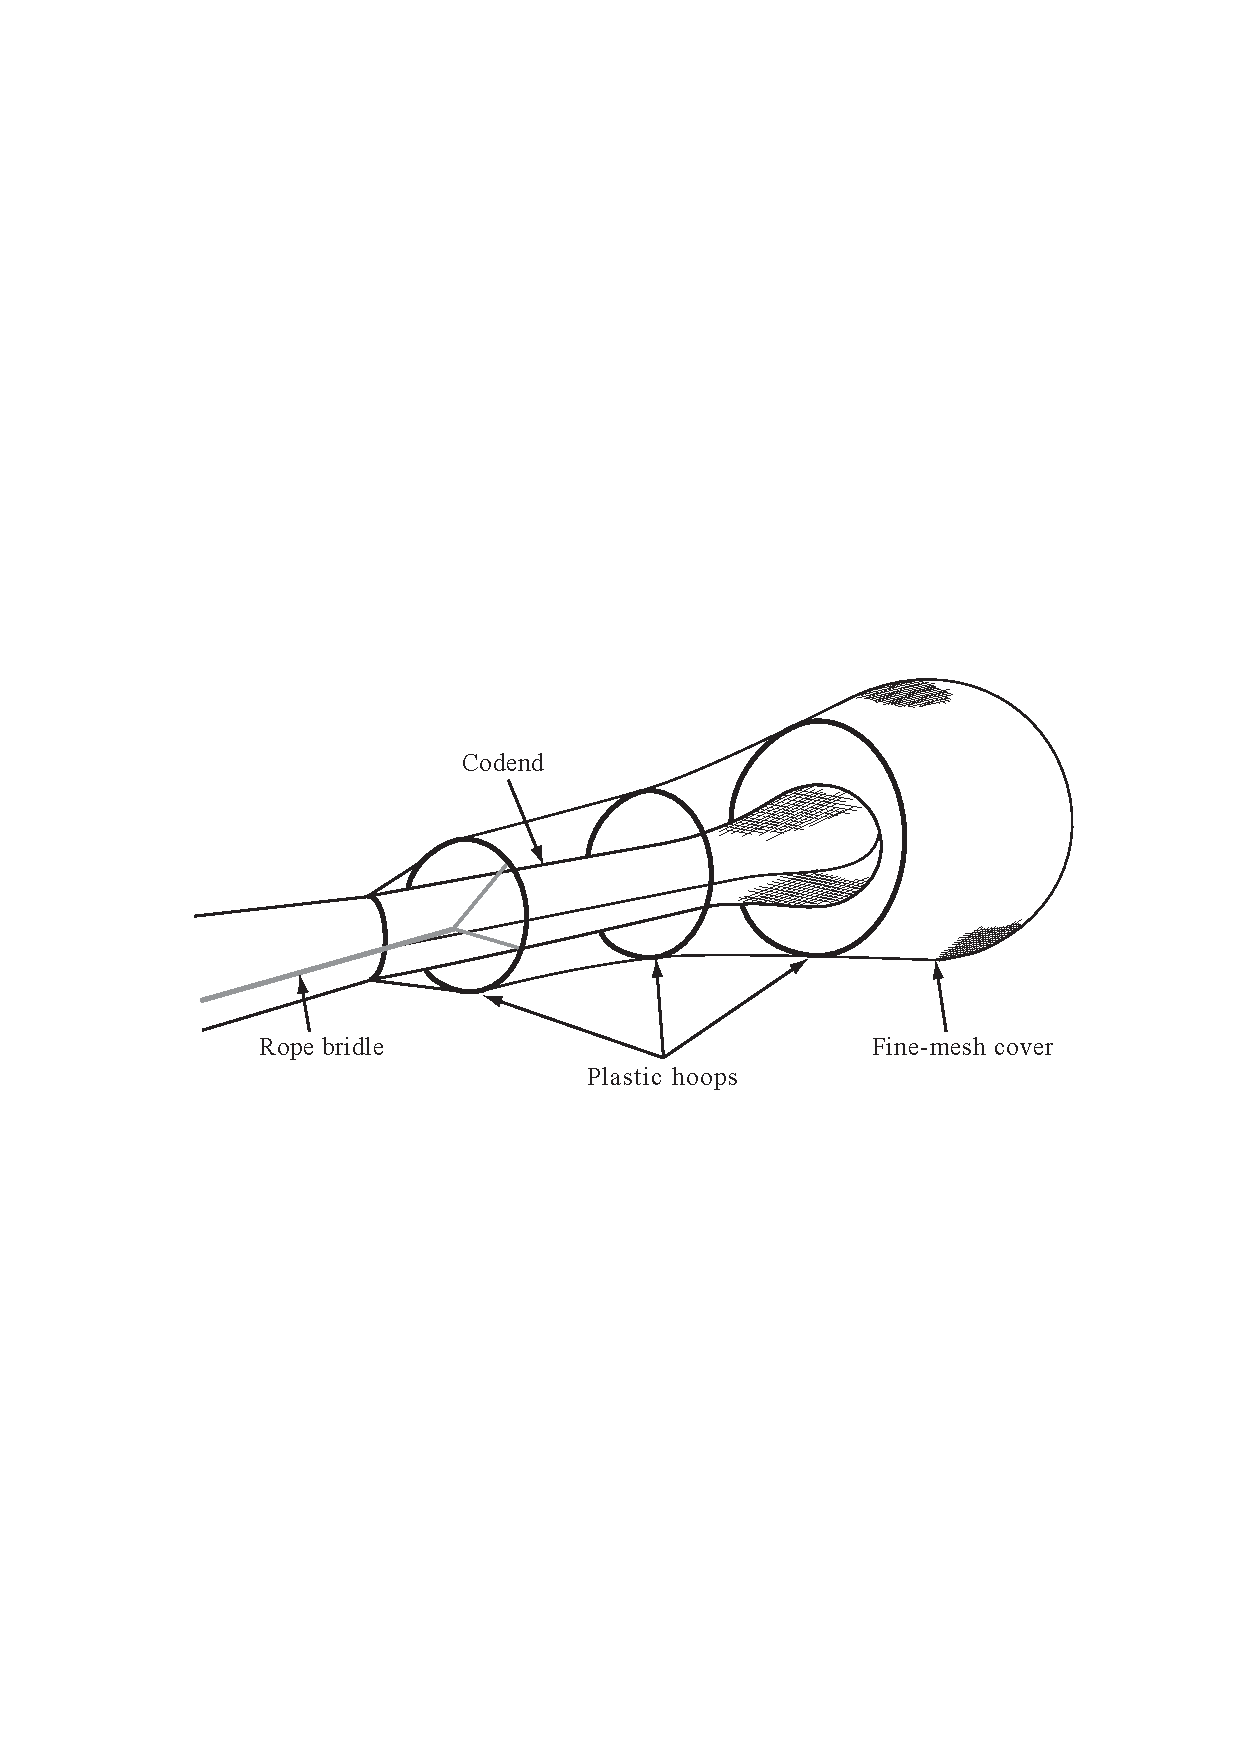
\includegraphics[width=4in]{Figures/CoveredCodendFig.pdf}
\end{center}
\end{frame}


\begin{frame}[fragile]
\frametitle{Fishing}
\begin{knitrout}\scriptsize
\definecolor{shadecolor}{rgb}{0.969, 0.969, 0.969}\color{fgcolor}\begin{kframe}
\begin{alltt}
\hlstd{> }\hlstd{Haddock.df} \hlkwb{=} \hlkwd{read.table}\hlstd{(}\hlstr{"Data/Haddock.dat"}\hlstd{,} \hlkwc{head} \hlstd{=} \hlnum{TRUE}\hlstd{)}
\hlstd{> }\hlstd{Haddock.df} \hlkwb{=} \hlkwd{transform}\hlstd{(Haddock.df,}\hlkwc{propn}\hlstd{=codend}\hlopt{/}\hlstd{(codend}\hlopt{+}\hlstd{cover))}
\hlstd{> }\hlkwd{head}\hlstd{(Haddock.df,} \hlnum{17}\hlstd{)}
\end{alltt}
\begin{verbatim}
   forklen codend cover      propn
1     19.5      0     2 0.00000000
2     20.5      0     5 0.00000000
3     21.5      0    11 0.00000000
4     22.5      0    28 0.00000000
5     23.5      1    53 0.01851852
6     24.5      5    46 0.09803922
7     25.5      1    35 0.02777778
8     26.5      3    27 0.10000000
9     27.5      1     5 0.16666667
10    28.5      0     3 0.00000000
11    29.5      1     2 0.33333333
12    30.5      0     0        NaN
13    31.5      0     2 0.00000000
14    32.5      3     2 0.60000000
15    33.5      4     4 0.50000000
16    34.5      5    12 0.29411765
17    35.5      8     9 0.47058824
\end{verbatim}
\end{kframe}
\end{knitrout}
\end{frame}


\begin{frame}[fragile]
\frametitle{Fishing\ldots}
\begin{knitrout}\scriptsize
\definecolor{shadecolor}{rgb}{0.969, 0.969, 0.969}\color{fgcolor}\begin{kframe}
\begin{alltt}
\hlstd{> }\hlkwd{tail}\hlstd{(Haddock.df,} \hlnum{20}\hlstd{)}
\end{alltt}
\begin{verbatim}
   forklen codend cover     propn
18    36.5     13    14 0.4814815
19    37.5     29    15 0.6590909
20    38.5     29     8 0.7837838
21    39.5     34     9 0.7906977
22    40.5     30     3 0.9090909
23    41.5     29     3 0.9062500
24    42.5     18     2 0.9000000
25    43.5     16     1 0.9411765
26    44.5     11     0 1.0000000
27    45.5     12     0 1.0000000
28    46.5      9     0 1.0000000
29    47.5      3     0 1.0000000
30    48.5      5     1 0.8333333
31    49.5      3     0 1.0000000
32    50.5      5     0 1.0000000
33    51.5      2     0 1.0000000
34    52.5      2     0 1.0000000
35    53.5      1     0 1.0000000
36    54.5      1     0 1.0000000
37    55.5      4     0 1.0000000
\end{verbatim}
\end{kframe}
\end{knitrout}
\end{frame}


\begin{frame}[fragile]
\frametitle{Fishing\ldots}
\framesubtitle{Plot the data}
\begin{knitrout}\scriptsize
\definecolor{shadecolor}{rgb}{0.969, 0.969, 0.969}\color{fgcolor}\begin{kframe}
\begin{alltt}
\hlstd{> }\hlkwd{plot}\hlstd{(propn} \hlopt{~} \hlstd{forklen,} \hlkwc{data} \hlstd{= Haddock.df,} \hlkwc{xlab} \hlstd{=} \hlstr{"Fork length (cm)"}\hlstd{)}
\end{alltt}
\end{kframe}
\end{knitrout}

\begin{figure}
  \centering
  \includegraphics{figure/RC-H15-036}
\end{figure}

Note that the proportions retained seem to follow an ``S'' shape.
\end{frame}


\begin{frame}[fragile]
\frametitle{Fishing\ldots}
\framesubtitle{Fitting the model}
Let's fit a logistic regression model. 
\bigskip

Note that the data are grouped, and the number of ``successes'' and ``failures'' are given by the variables \rcode{codend} and \rcode{cover}, respectively\footnote{Retaining the fish may by a success for the fisherman, but perhaps not for the fish!}. 
\bigskip

\begin{knitrout}\scriptsize
\definecolor{shadecolor}{rgb}{0.969, 0.969, 0.969}\color{fgcolor}\begin{kframe}
\begin{alltt}
\hlstd{> }\hlstd{Haddock.glm} \hlkwb{=} \hlkwd{glm}\hlstd{(}\hlkwd{cbind}\hlstd{(codend,cover)} \hlopt{~} \hlstd{forklen,} \hlkwc{family} \hlstd{= binomial,}
\hlstd{+ }                  \hlkwc{data} \hlstd{= Haddock.df)}
\end{alltt}
\end{kframe}
\end{knitrout}

\end{frame}


\begin{frame}[fragile]
\frametitle{Fishing\ldots}
\framesubtitle{Modelling proportion data using log-odds}
%\framesubtitle{Logistic regression using glm}
\begin{knitrout}\scriptsize
\definecolor{shadecolor}{rgb}{0.969, 0.969, 0.969}\color{fgcolor}\begin{kframe}
\begin{alltt}
\hlstd{> }\hlkwd{summary}\hlstd{(Haddock.glm)}
\end{alltt}
\end{kframe}
\end{knitrout}

\begin{knitrout}\scriptsize
\definecolor{shadecolor}{rgb}{0.969, 0.969, 0.969}\color{fgcolor}\begin{kframe}
\begin{verbatim}
Call:
glm(formula = cbind(codend, cover) ~ forklen, family = binomial, 

Coefficients:
             Estimate Std. Error z value Pr(>|z|)    
(Intercept) -10.63219    0.86468  -12.30   <2e-16 ***
forklen       0.30396    0.02363   12.86   <2e-16 ***
---
(Dispersion parameter for binomial family taken to be 1)

    Null deviance: 432.464  on 35  degrees of freedom
Residual deviance:  23.436  on 34  degrees of freedom
\end{verbatim}
\end{kframe}
\end{knitrout}
\end{frame}


\begin{frame}[fragile]
\frametitle{Fishing\ldots}
\framesubtitle{Checking the fitted model}

As with the Poisson case, we need to check the residual deviance by comparing it to a $\chi^2$ distribution. We can do this here as the data are grouped: we have many observations for each level of fork-length, so the data are not `sparse'.

\medskip

The residual deviance is 23.44 on 34 degrees of freedom. 
The \pval{} is 

\begin{knitrout}\scriptsize
\definecolor{shadecolor}{rgb}{0.969, 0.969, 0.969}\color{fgcolor}\begin{kframe}
\begin{alltt}
\hlstd{> }\hlnum{1}\hlopt{-}\hlkwd{pchisq}\hlstd{(}\hlnum{23.44}\hlstd{,}\hlnum{34}\hlstd{)}
\end{alltt}
\begin{verbatim}
[1] 0.9132025
\end{verbatim}
\end{kframe}
\end{knitrout}
which indicates no significant problems with the fitted model.

\bigskip
{\bf Recall:} 
If the residual deviance indicated lack of fit then we would have to refit
using \rcode{family = quasibinomial}.
\end{frame}



\begin{frame}[fragile]
\frametitle{Fishing\ldots}
\framesubtitle{Checking the fitted model\ldots}
Let's check the residual plot
\begin{knitrout}\scriptsize
\definecolor{shadecolor}{rgb}{0.969, 0.969, 0.969}\color{fgcolor}\begin{kframe}
\begin{alltt}
\hlstd{> }\hlkwd{plot}\hlstd{(Haddock.glm,}\hlkwc{which}\hlstd{=}\hlnum{1}\hlstd{,} \hlkwc{lty}\hlstd{=}\hlnum{2}\hlstd{)}
\end{alltt}
\end{kframe}
\end{knitrout}

\begin{figure}
  \centering
  \includegraphics{figure/RC-H15-041}
\end{figure}

Looks good, other than one largish residual corresponding to the 48.5 cm fish that was in the cover.
\end{frame}



\begin{frame}[fragile]
\frametitle{Fishing\ldots}
\framesubtitle{Checking the fitted model\ldots}
Lets check the influence plot
\begin{knitrout}\scriptsize
\definecolor{shadecolor}{rgb}{0.969, 0.969, 0.969}\color{fgcolor}\begin{kframe}
\begin{alltt}
\hlstd{> }\hlkwd{plot}\hlstd{(Haddock.glm,}\hlkwc{which}\hlstd{=}\hlnum{4}\hlstd{)}
\end{alltt}
\end{kframe}
\end{knitrout}

\begin{figure}
  \centering
  \includegraphics{figure/RC-H15-041b}
\end{figure}

Hmmm, the fit is somewhat influenced by the retention of small fish of length 24.5 cm. However, this is known to happen with trawl gear, so this observation will not be removed.
\end{frame}



\begin{frame}[fragile]
% \frametitle{Modeling proportion data using log-odds\ldots}
\frametitle{Fishing\ldots}
\framesubtitle{Interpretation}
\begin{knitrout}\scriptsize
\definecolor{shadecolor}{rgb}{0.969, 0.969, 0.969}\color{fgcolor}\begin{kframe}
\begin{alltt}
\hlstd{> }  \hlkwd{summary}\hlstd{(Haddock.glm)}\hlopt{$}\hlstd{coef}
\end{alltt}
\begin{verbatim}
               Estimate Std. Error   z value     Pr(>|z|)
(Intercept) -10.6321889 0.86467598 -12.29615 9.499049e-35
forklen       0.3039569 0.02363082  12.86273 7.295469e-38
\end{verbatim}
\end{kframe}
\end{knitrout}
Remember, the linear model is on the log-odds scale.
So, the value 0.304 corresponds to an estimated increase in the log-odds of codend retention for every one cm increase in \rcode{forklen}.

\bigskip

The 95\% confidence intervals for $\beta_0$ and $\beta_1$ are:
\begin{knitrout}\scriptsize
\definecolor{shadecolor}{rgb}{0.969, 0.969, 0.969}\color{fgcolor}\begin{kframe}
\begin{alltt}
\hlstd{> }  \hlkwd{confint}\hlstd{(Haddock.glm)}
\end{alltt}


{\ttfamily\noindent\itshape\color{messagecolor}{Waiting for profiling to be done...}}\begin{verbatim}
                  2.5 %     97.5 %
(Intercept) -12.4563256 -9.0501022
forklen       0.2604867  0.3535532
\end{verbatim}
\end{kframe}
\end{knitrout}
\end{frame}



\begin{frame}[fragile]
% \frametitle{Modeling proportion data using log-odds\ldots}
\frametitle{Fishing\ldots}
\framesubtitle{Interpretation\ldots}
Exponentiating the above confidence intervals gives:
\begin{knitrout}\scriptsize
\definecolor{shadecolor}{rgb}{0.969, 0.969, 0.969}\color{fgcolor}\begin{kframe}
\begin{alltt}
\hlstd{> }\hlkwd{exp}\hlstd{(}\hlkwd{confint}\hlstd{(Haddock.glm))}
\end{alltt}


{\ttfamily\noindent\itshape\color{messagecolor}{Waiting for profiling to be done...}}\begin{verbatim}
                   2.5 %      97.5 %
(Intercept) 3.893019e-06 0.000117379
forklen     1.297561e+00 1.424118770
\end{verbatim}
\end{kframe}
\end{knitrout}



\medskip

In our {\bf Executive Summary} we could say something like 
\medskip

``Every 1 cm increase in the fork length of a haddock multiplies the odds of it being retained in the codend by between 1.3 and 1.42".
\medskip

Or, ``Every 1 cm increase in the fork length of a haddock corresponds to an increase
in odds of it being retained in the codend of between 30\% and 42\%".
\end{frame}


\begin{frame}[fragile]
% \frametitle{Fishing example}
\frametitle{Fishing\ldots}

Here is a plot of the data with the fitted ``S" curve overlaid:


\begin{figure}
  % \centering
  \includegraphics{figure/RC-H15-046}
\end{figure}

\end{frame}


\begin{frame}[fragile]
\frametitle{Fishing\ldots}
\framesubtitle{Confidence intervals for $p$}
To estimate the probability of retention for haddock of lengths 25, 35 and 45 cm:
\bigskip

\begin{knitrout}\scriptsize
\definecolor{shadecolor}{rgb}{0.969, 0.969, 0.969}\color{fgcolor}\begin{kframe}
\begin{alltt}
\hlstd{> }\hlstd{predn}\hlkwb{=}\hlkwd{predictGLM}\hlstd{(Haddock.glm,} \hlkwd{data.frame}\hlstd{(}\hlkwc{forklen}\hlstd{=}\hlkwd{c}\hlstd{(}\hlnum{25}\hlstd{,}\hlnum{35}\hlstd{,}\hlnum{45}\hlstd{)),} \hlkwc{type}\hlstd{=}\hlstr{"response"}\hlstd{)}
\end{alltt}


{\ttfamily\noindent\itshape\color{messagecolor}{***Estimates and CIs are on the response scale***}}\begin{alltt}
\hlstd{> }\hlstd{predn}
\end{alltt}
\begin{verbatim}
         fit        lwr        upr
1 0.04594542 0.02639853 0.07879451
2 0.50157550 0.43868954 0.56441166
3 0.95460393 0.92887749 0.97131200
\end{verbatim}
\end{kframe}
\end{knitrout}
\bigskip

The probability that a 25 cm haddock is retained in the codend is between 0.026 and 0.079. This increases to between 0.439 and 0.564 for 35 cm haddock, and between 0.929 and 0.971 for 45 cm haddock.


\end{frame}



%%%%%%%%%%%%%%%%%%%%%%%%%%%%%%%%%%%%%%%%%%%%%%%%%%%%%%%%%%%%%%%%%%%%%%%%%%%%%%%%%%%%%%%%%%%
\BeginSection{Relevant \rcode{R}-code.}
%%%%%%%%%%%%%%%%%%%%%%%%%%%%%%%%%%%%%%%%%%%%%%%%%%%%%%%%%%%%%%%%%%%%%%%%%%%%%%%%%%%%%%%%%%%


\begin{frame}[fragile]
\frametitle{Most of the \rcode{R}-code you need for this chapter}

{\bf Ungrouped data}
\medskip

Ungrouped data are binary i.e., a 0 or 1 response value for each observation (for example \rcode{bb.df}). Fit the model with \rcode{glm} using \rcode{family=binomial}:

\begin{knitrout}\scriptsize
\definecolor{shadecolor}{rgb}{0.969, 0.969, 0.969}\color{fgcolor}\begin{kframe}
\begin{alltt}
\hlstd{> }\hlstd{bb.fit2} \hlkwb{=} \hlkwd{glm}\hlstd{(basket} \hlopt{~} \hlstd{distance,} \hlkwc{family} \hlstd{= binomial,} \hlkwc{data} \hlstd{= bb.df)}
\end{alltt}
\end{kframe}
\end{knitrout}

These type of data are known as sparse  (because either the count of successes is 0 or the count of failures is 0) and we cannot test our model assumptions effectively as we would like to. If possible we should group our data.
\end{frame}



\begin{frame}[fragile]
\frametitle{Most of the \rcode{R}-code you need for this chapter\ldots}

{\bf Grouped data}
\medskip

We were also able to analyse the basketball data as grouped observations which allows us to check assumptions including if we have to make a \rcode{family= quasibinomial} adjustment to our model.

\bigskip

{\bf Syntax 1} - specify proportion of successes and number of trials

\begin{knitrout}\scriptsize
\definecolor{shadecolor}{rgb}{0.969, 0.969, 0.969}\color{fgcolor}\begin{kframe}
\begin{alltt}
\hlstd{> }\hlstd{bb.fit3} \hlkwb{=} \hlkwd{glm}\hlstd{(propn} \hlopt{~} \hlstd{distance} \hlopt{*} \hlstd{gender,}\hlkwc{weight}\hlstd{=n,}
\hlstd{+ }              \hlkwc{family} \hlstd{= binomial,}\hlkwc{data} \hlstd{= bb.grouped.df)}
\end{alltt}
\end{kframe}
\end{knitrout}

{\bf Syntax 2} - specify frequency of successes and failures

\begin{knitrout}\scriptsize
\definecolor{shadecolor}{rgb}{0.969, 0.969, 0.969}\color{fgcolor}\begin{kframe}
\begin{alltt}
\hlstd{> }\hlstd{bb.grouped.df} \hlkwb{=} \hlkwd{transform}\hlstd{(bb.grouped.df,} \hlkwc{success}\hlstd{=n}\hlopt{*}\hlstd{propn,} \hlkwc{fail}\hlstd{=n}\hlopt{*}\hlstd{(}\hlnum{1}\hlopt{-}\hlstd{propn))}
\hlstd{> }\hlstd{bb.fit4} \hlkwb{=} \hlkwd{glm}\hlstd{(}\hlkwd{cbind}\hlstd{(success, fail)} \hlopt{~} \hlstd{distance} \hlopt{*} \hlstd{gender,}
\hlstd{+ }              \hlkwc{family} \hlstd{= binomial,}\hlkwc{data} \hlstd{= bb.grouped.df)}
\end{alltt}
\end{kframe}
\end{knitrout}

\end{frame}



\begin{frame}[fragile]
\frametitle{Most of the \rcode{R}-code you need for this chapter\ldots}
Both model syntaxs give exactly the same results and we can perform the residual deviance check as follows:
\medskip

\begin{knitrout}\scriptsize
\definecolor{shadecolor}{rgb}{0.969, 0.969, 0.969}\color{fgcolor}\begin{kframe}
\begin{alltt}
\hlstd{> }\hlnum{1}\hlopt{-}\hlkwd{pchisq}\hlstd{(bb.fit4}\hlopt{$}\hlstd{deviance,bb.fit4}\hlopt{$}\hlstd{df.residual)}
\hlstd{> }\hlcom{# or directly}
\hlstd{> }\hlnum{1} \hlopt{-} \hlkwd{pchisq}\hlstd{(}\hlnum{2.3688}\hlstd{,} \hlnum{2}\hlstd{)}
\end{alltt}
\end{kframe}
\end{knitrout}
\bigskip

If the p-value is below 0.05 then we have evidence against the assumed binomial distribution
and need to refit our model using \rcode{family= quasibinomial}.
\end{frame}



\begin{frame}[fragile]
\frametitle{Most of the \rcode{R}-code you need for this chapter\ldots}
Confidence intervals can be calculated for the parameters and back-transformed and interpreted as a  multiplicative effect on the odds (or as a \% change if you prefer).

\begin{knitrout}\scriptsize
\definecolor{shadecolor}{rgb}{0.969, 0.969, 0.969}\color{fgcolor}\begin{kframe}
\begin{alltt}
\hlstd{> }\hlstd{(bb.ci2} \hlkwb{=} \hlkwd{confint}\hlstd{(bb.fit2))}
\hlstd{> }\hlkwd{exp}\hlstd{(bb.ci2)}
\end{alltt}
\end{kframe}
\end{knitrout}
\bigskip 

Confidence intervals for probabilities take a bit more effort since they
require calcuating a confidence interval on the logit scale (i.e., for log-odds) and then backtransforming using the logistic function. 
\medskip

Fortunately, we can use \rcode{predictGLM}.

\begin{knitrout}\scriptsize
\definecolor{shadecolor}{rgb}{0.969, 0.969, 0.969}\color{fgcolor}\begin{kframe}
\begin{alltt}
\hlstd{> }\hlstd{bb.pred.intervals} \hlkwb{=} \hlkwd{predictGLM}\hlstd{(bb.fit2,}
\hlstd{+ }                            \hlkwc{newdata} \hlstd{=} \hlkwd{data.frame}\hlstd{(}\hlkwc{distance} \hlstd{=} \hlkwd{c}\hlstd{(}\hlnum{1}\hlstd{,} \hlnum{2}\hlstd{,} \hlnum{3}\hlstd{)),}
\hlstd{+ }                            \hlkwc{type}\hlstd{=}\hlstr{"response"}\hlstd{)}
\end{alltt}


{\ttfamily\noindent\itshape\color{messagecolor}{***Estimates and CIs are on the response scale***}}\begin{alltt}
\hlstd{> }\hlstd{bb.pred.intervals}
\end{alltt}
\begin{verbatim}
        fit        lwr       upr
1 0.9595708 0.82769294 0.9915450
2 0.6308584 0.44733881 0.7829992
3 0.1095708 0.03370437 0.3027108
\end{verbatim}
\end{kframe}
\end{knitrout}
 
\end{frame}



\end{document}
